% =====================================================================
\chapter{\emph{Backtest} rigoureux}
\label{ch:16}
% =====================================================================

\section{Objectifs et organisation du chapitre}

\paragraph{Objectifs.} Un \emph{backtest} rejoue une stratégie sur des données passées pour estimer ce qu'elle aurait rapporté. C'est l'outil central du trader quantitatif, et c'est aussi le meilleur moyen de se mentir. À la fin du chapitre, vous saurez : (1) reconnaître et éliminer les biais d'anticipation, de survie et de sélection ; (2) organiser formation, validation et test sans fuite d'information ; (3) calculer l'erreur-type d'un ratio de Sharpe et savoir combien d'années il faut pour distinguer un bon Sharpe du hasard ; (4) corriger un Sharpe du nombre de variantes essayées (ratio de Sharpe déflaté) ; (5) estimer la probabilité qu'une optimisation soit du surapprentissage (PBO) ; (6) utiliser le moteur de \emph{backtest} du paquet \texttt{arbhub}, testé contre l'anticipation.

\paragraph{Code.} \texttt{code/ch16/ch16\_backtest.py} (expériences E1 à E6), et les modules réutilisables \texttt{src/arbhub/backtest/engine.py} et \texttt{metrics.py}, avec leurs tests dans \texttt{tests/test\_backtest.py}.

\begin{intuition}
Un \emph{backtest}, c'est un examen blanc dont vous auriez écrit vous-même le sujet. Si vous avez vu les réponses en écrivant le sujet (anticipation), si vous n'avez gardé que les copies des élèves qui ont réussi l'année (survie), ou si vous avez passé l'examen cinquante fois en ne retenant que la meilleure note (sélection), la note ne dit rien de ce qui se passera le jour du vrai examen. Tout ce chapitre consiste à rendre l'examen blanc aussi honnête que le vrai.
\end{intuition}

% =====================================================================
\section{Les trois biais fatals}
% =====================================================================

\subsection{Le biais d'anticipation}

\begin{definition}
Un \emph{backtest} souffre d'un \emph{biais d'anticipation} (\emph{look-ahead bias}) si une décision datée de $t$ utilise, même indirectement, une information qui n'était pas disponible à la date $t$.
\end{definition}

Les formes les plus fréquentes en arbitrage statistique sont :
\begin{enumerate}
\item \textbf{la position appliquée trop tôt :} la position décidée avec le prix de clôture de $t$ est appliquée à la variation de $t-1$ à $t$, alors qu'on ne pouvait la prendre qu'\emph{à} la clôture de $t$ ;
\item \textbf{la normalisation globale :} le \emph{z-score} est calculé avec la moyenne et l'écart-type de \emph{toute} la période ; à la date $t$, on \og sait\fg{} donc déjà autour de quel niveau l'écart finira ;
\item \textbf{le ratio de couverture global :} $\beta$ est estimé par régression sur toute la période, puis utilisé dès le premier jour ;
\item \textbf{les données révisées ou ajustées :} prix ajustés des dividendes ou des divisions calculés après coup, compositions d'indices connues après coup, données macroéconomiques révisées.
\end{enumerate}

La règle qui élimine les trois premières est celle du chapitre~1, écrite une fois pour toutes dans le moteur :
\begin{equation}\label{c16:eq:pnl}
\text{gain}_{t+1} = q_t\,(S_{t+1} - S_t), \qquad q_t = f\big(\text{données datées} \le t\big),
\end{equation}
et tous les paramètres ($\beta$, moyenne, écart-type, seuils) sont estimés soit sur une période de formation \emph{antérieure}, soit en fenêtre glissante \emph{strictement passée}.

\begin{codebox}[ — E1, un écart sans avantage rejoué de quatre façons]
\textbf{Protocole :} 300 mondes de 1\,000 jours où l'écart $y - 1{,}5x$ est une \emph{marche aléatoire} : aucune stratégie de retour à la moyenne ne peut y gagner en espérance. Règle $|z|>2$, sortie à $z=0$, \emph{z-score} glissant sur 60 jours, sans coûts. \textbf{Sharpe annualisé médian (part des mondes gagnants) :}
\begin{center}\small
\begin{tabular}{lcc}
\toprule
Implémentation & Sharpe médian & Mondes gagnants \\
\midrule
Correcte (équation~\ref{c16:eq:pnl}) & $0{,}07$ & 54,7\,\% \\
$\beta$ estimé sur toute la période & $0{,}24$ & 66,7\,\% \\
Moyenne et écart-type de toute la période & $0{,}85$ & 77,7\,\% \\
Position appliquée le jour même & $-0{,}89$ & 0,7\,\% \\
\bottomrule
\end{tabular}
\end{center}
Dans un monde \emph{avec} avantage ($\varphi = 0{,}97$), l'implémentation correcte donne un Sharpe médian de $1{,}09$ et la position appliquée le jour même $-0{,}13$.
\end{codebox}

\begin{figure}[h]
\centering
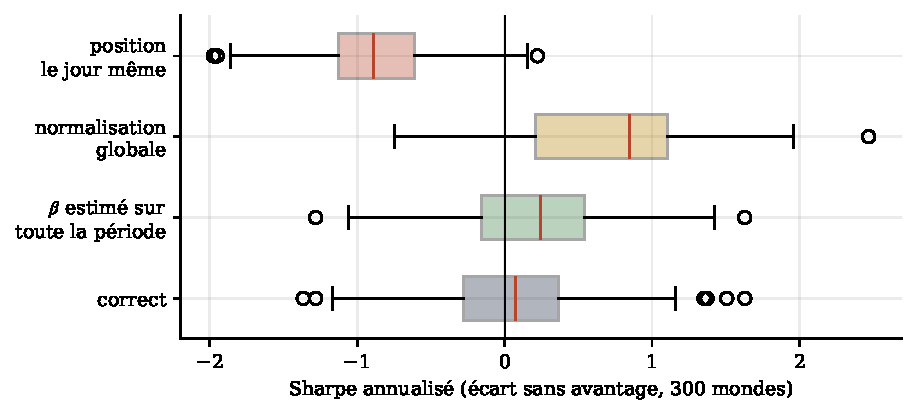
\includegraphics[width=0.72\textwidth]{ch16/biais_anticipation.pdf}
\caption{Distribution du Sharpe annualisé sur 300 mondes sans avantage, selon l'implémentation. Seule la version correcte est centrée sur zéro.}
\label{c16:fig:lookahead}
\end{figure}

\paragraph{Lecture.} La normalisation globale fabrique un Sharpe de $0{,}85$ à partir de rien : en connaissant le niveau moyen final de l'écart, on sait dans quel sens il finira par \og revenir\fg. Le $\beta$ global fait la même chose plus discrètement. L'erreur de date donne un résultat très \emph{négatif} : pour une stratégie contrariante, la position décidée en voyant un écart monter est une vente, et l'appliquer à la hausse qui vient d'avoir lieu fait perdre. Le biais d'anticipation n'a donc pas de signe fixe ; il rend simplement le résultat faux. Un \emph{backtest} anormalement mauvais mérite la même méfiance qu'un \emph{backtest} anormalement bon.

\begin{pitfall}
Le test le plus efficace contre l'anticipation n'est pas la relecture du code, c'est un test automatique : on modifie toutes les données \emph{après} une date $t_0$ et l'on vérifie que les positions et le P\&L jusqu'à $t_0$ sont inchangés. C'est le test \texttt{test\_no\_lookahead\_signal\_and\_pnl} du dépôt ; le fichier \texttt{CLAUDE.md} en exige un pour chaque nouvelle stratégie.
\end{pitfall}

\subsection{Le biais de survie}

\begin{definition}
Il y a \emph{biais de survie} quand l'univers testé ne contient que les actifs qui existent encore aujourd'hui, en excluant ceux qui ont été radiés (faillite, rachat, fusion) pendant la période.
\end{definition}

En \emph{pairs trading}, c'est particulièrement grave : une paire se rompt souvent \emph{parce que} l'une des deux sociétés subit un événement qui finit par sa radiation. Exclure les radiées revient à exclure précisément les paires qui ont perdu.

\begin{codebox}[ — E6, biais de survie]
\textbf{Protocole :} 400 paires ; 30\,\% d'entre elles subissent une rupture (l'écart se met à dériver durablement) et l'action concernée est radiée 100 jours plus tard ; règle $|z|>2$ calibrée sur 500 jours, coûts 5 pb par jambe. \textbf{Résultats :} 303 paires survivent. Sur toutes les paires, gain moyen $52{,}05$ et Sharpe médian $1{,}92$ ; sur les seules survivantes, gain moyen $62{,}86$ (+21\,\%) et Sharpe médian $2{,}03$.
\end{codebox}

La correction consiste à utiliser une base de données qui conserve les titres radiés avec leur dernier prix, et à reconstituer l'univers \emph{tel qu'il était connu à chaque date} (\emph{point-in-time}).

\subsection{Le biais de sélection et les tests multiples}

\begin{intuition}
Lancez 1\,000 pièces de monnaie dix fois chacune. Une dizaine d'entre elles feront au moins neuf \og pile\fg{} sur dix. Ce ne sont pas des pièces truquées : c'est ce qui arrive quand on regarde 1\,000 pièces. Essayer 1\,000 paires, 50 seuils ou 20 fenêtres et retenir la meilleure combinaison, c'est exactement la même chose.
\end{intuition}

Le reste du chapitre quantifie ce biais. Il faut d'abord savoir à quel point un ratio de Sharpe est imprécis, même sans sélection.

% =====================================================================
\section{L'erreur d'estimation du ratio de Sharpe}
% =====================================================================

\subsection{Définition}

Pour des rendements (ou gains) par période $r_1,\dots,r_T$, le ratio de Sharpe par période est $\widehat{SR} = \bar r/\hat s$, où $\bar r$ est la moyenne et $\hat s$ l'écart-type. Le Sharpe annualisé vaut $\widehat{SR}\sqrt{P}$, avec $P$ le nombre de périodes par an (252 en données quotidiennes). Pour une stratégie de paires, on calcule le Sharpe des gains nets rapportés au capital engagé, ou directement des gains en devise : le ratio est le même à un facteur d'échelle près.

\subsection{Erreur-type}

\begin{proposition}[\citet{lo2002}]\label{c16:prop:sese}
Si les rendements sont i.i.d. de loi normale, l'estimateur $\widehat{SR}$ est asymptotiquement normal, d'espérance $SR$ et d'écart-type
\[
\operatorname{se}(\widehat{SR}) \approx \sqrt{\frac{1 + \frac12 SR^2}{T}}.
\]
Pour des rendements i.i.d. non normaux d'asymétrie $\gamma_3$ et de kurtosis $\gamma_4$ (égale à 3 pour la loi normale), la formule devient $\sqrt{\big(1 - \gamma_3 SR + \frac{\gamma_4-1}{4}SR^2\big)/T}$ \citep{bailey2014dsr}.
\end{proposition}
\begin{proof}[Idée de la démonstration]
$\widehat{SR}$ est une fonction $g(\bar r, \hat s^2) = \bar r/\sqrt{\hat s^2}$ des deux premiers moments empiriques. Pour une loi normale, $\bar r$ et $\hat s^2$ sont indépendants, de variances $s^2/T$ et $2s^4/T$. La méthode delta donne $\Var(\widehat{SR}) \approx (\partial_1 g)^2\,s^2/T + (\partial_2 g)^2\,2s^4/T$, avec $\partial_1 g = 1/s$ et $\partial_2 g = -\bar r/(2s^3)$. D'où $\Var(\widehat{SR}) \approx 1/T + (\bar r^2/(4s^6))\,2s^4/T = (1 + SR^2/2)/T$.
\end{proof}

\paragraph{Conséquence pratique.} Le terme $SR^2/2$ est négligeable en données quotidiennes (un Sharpe annuel de 1 correspond à $SR = 1/\sqrt{252} \approx 0{,}063$ par jour). L'erreur-type du Sharpe \emph{annualisé} vaut donc environ $\sqrt{252/T} = 1/\sqrt{\text{nombre d'années}}$.

\begin{codebox}[ — E2, dispersion du Sharpe estimé d'une stratégie de vrai Sharpe annuel 1]
\textbf{Protocole :} 4\,000 simulations par durée, rendements normaux puis de Student à 4 degrés de liberté (queues épaisses). \textbf{Écart-type du Sharpe annualisé estimé :}
\begin{center}\small
\begin{tabular}{rcccc}
\toprule
Durée & Normal & Formule de Lo & Student(4) & Intervalle à 95\,\% (normal) \\
\midrule
1 an & 0,981 & 1,003 & 1,012 & $[-0{,}92\,;\,2{,}92]$ \\
3 ans & 0,581 & 0,578 & 0,580 & $[-0{,}14\,;\,2{,}14]$ \\
5 ans & 0,442 & 0,448 & 0,447 & $[0{,}13\,;\,1{,}87]$ \\
10 ans & 0,316 & 0,317 & 0,316 & $[0{,}38\,;\,1{,}62]$ \\
\bottomrule
\end{tabular}
\end{center}
\end{codebox}

\paragraph{Lecture.} Avec un an de données, une stratégie de vrai Sharpe 1 affiche un Sharpe estimé n'importe où entre $-0{,}9$ et $2{,}9$. Il faut environ cinq ans pour que l'intervalle à 95\,\% exclue zéro. En données quotidiennes, les queues épaisses changent très peu l'erreur-type (le terme en $\gamma_4$ est multiplié par $SR^2$, minuscule) ; elles comptent davantage pour des rendements mensuels ou pour des stratégies à gains rares et pertes extrêmes.

\begin{pitfall}
La formule suppose des rendements indépendants. Les gains quotidiens d'une stratégie de paires sont autocorrélés (on reste plusieurs jours en position) : l'erreur-type réelle est plus grande. On peut l'estimer par un \emph{bootstrap} par blocs ou avec un estimateur de variance robuste à l'autocorrélation \citep{neweywest1987}.
\end{pitfall}

% =====================================================================
\section{Le maximum de plusieurs Sharpe}
% =====================================================================

On essaie $N$ variantes indépendantes d'une stratégie qui n'ont \emph{aucun} avantage (vrai Sharpe nul), et on garde la meilleure. Quel Sharpe affichera-t-elle en moyenne ?

\begin{proposition}[\citet{bailey2014dsr}]\label{c16:prop:emax}
Si les $N$ Sharpe estimés sont indépendants, de loi approximativement $\N(0, V)$, alors
\[
\E\Big[\max_{1\le n\le N}\widehat{SR}_n\Big] \approx \sqrt V\,\Big((1-\gamma)\,\Phi^{-1}\!\Big(1-\frac1N\Big) + \gamma\,\Phi^{-1}\!\Big(1-\frac{1}{N e}\Big)\Big),
\]
où $\gamma \approx 0{,}5772$ est la constante d'Euler-Mascheroni et $\Phi^{-1}$ la fonction quantile de la loi normale.
\end{proposition}
\begin{proof}[Idée]
Le maximum de $N$ variables normales indépendantes se concentre autour du quantile $1-1/N$ ; la théorie des valeurs extrêmes (loi de Gumbel, dont l'espérance fait apparaître $\gamma$) fournit la correction entre les deux quantiles.
\end{proof}

Avec $V = 1/T$ (proposition~\ref{c16:prop:sese} pour $SR=0$), le maximum croît comme $\sqrt{2\ln N/T}$ : lentement, mais sans limite.

\begin{codebox}[ — E3, meilleur Sharpe annualisé parmi $N$ stratégies sans avantage, 3 ans de données]
\begin{center}\small
\begin{tabular}{rccccccc}
\toprule
$N$ & 1 & 5 & 10 & 50 & 100 & 500 & 1\,000 \\
\midrule
Simulation (200 tirages) & $-0{,}07$ & 0,69 & 0,87 & 1,32 & 1,46 & 1,78 & 1,89 \\
Formule & 0 & 0,69 & 0,91 & 1,32 & 1,46 & 1,76 & 1,88 \\
\bottomrule
\end{tabular}
\end{center}
\end{codebox}

\begin{figure}[h]
\centering
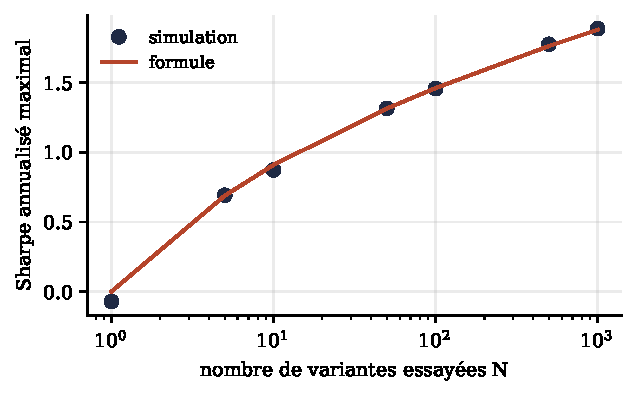
\includegraphics[width=0.55\textwidth]{ch16/max_sharpe.pdf}
\caption{Sharpe annualisé maximal attendu parmi $N$ stratégies sans avantage, sur 3 ans de données quotidiennes.}
\label{c16:fig:emax}
\end{figure}

\paragraph{Lecture.} En essayant 100 paires ou 100 réglages sur trois ans de données, on obtient \emph{en moyenne} un Sharpe de $1{,}46$ sans aucun avantage réel. C'est l'ordre de grandeur des performances publiées sur les réseaux sociaux. \citet{harvey2016} tirent la même conclusion pour la recherche académique : après des centaines de facteurs testés, un seuil de $t$-statistique de 2 est trop faible ; ils recommandent au moins 3.

% =====================================================================
\section{Le ratio de Sharpe probabiliste et déflaté}
% =====================================================================

\begin{definition}[PSR]
Le \emph{ratio de Sharpe probabiliste} d'un Sharpe estimé $\widehat{SR}$ sur $T$ périodes par rapport à un seuil $SR^\ast$ est
\[
\text{PSR}(SR^\ast) = \Phi\!\left(\frac{(\widehat{SR} - SR^\ast)\sqrt{T-1}}{\sqrt{1 - \gamma_3\widehat{SR} + \frac{\gamma_4-1}{4}\widehat{SR}^2}}\right).
\]
C'est la probabilité, compte tenu de l'erreur d'estimation (proposition~\ref{c16:prop:sese}), que le vrai Sharpe dépasse $SR^\ast$.
\end{definition}

\begin{definition}[DSR, \citet{bailey2014dsr}]
Le \emph{ratio de Sharpe déflaté} de la meilleure de $N$ variantes est le PSR calculé avec, pour seuil, le maximum espéré de la proposition~\ref{c16:prop:emax} : $\text{DSR} = \text{PSR}\big(\E[\max_n \widehat{SR}_n]\big)$, où $V$ est estimée par la variance des Sharpe des $N$ variantes essayées.
\end{definition}

\begin{intuition}
Le DSR répond à la question : \og ma meilleure variante bat-elle ce que le hasard m'aurait donné en essayant autant de variantes ?\fg. Un DSR supérieur à 0,95 signifie qu'il y a moins de 5\,\% de chances que le résultat ne soit que le meilleur tirage d'une loterie.
\end{intuition}

\begin{pitfall}
Le DSR exige de connaître $N$, le nombre de variantes \emph{réellement} essayées, y compris celles qu'on a abandonnées en cours de route, les autres paires regardées, les autres périodes testées. C'est pourquoi le fichier \texttt{CLAUDE.md} du dépôt impose de consigner le nombre de variantes avec chaque résultat. Si les variantes sont très corrélées (deux seuils voisins), $N$ \og effectif\fg{} est plus petit que le nombre brut : le DSR calculé avec le nombre brut est alors conservateur.
\end{pitfall}

% =====================================================================
\section{Organiser les données : formation, validation, test}
% =====================================================================

\subsection{Le découpage}

\begin{center}\small
\begin{tabular}{p{3.0cm}p{9.8cm}}
\toprule
Période & Usage \\
\midrule
Formation & Estimer les paramètres du modèle ($\beta$, moyenne, écart-type, demi-vie) et sélectionner les paires. \\
Validation & Choisir les réglages (seuil d'entrée, fenêtre) parmi un petit nombre de variantes déclarées à l'avance. \\
Test & Mesurer la performance \emph{une seule fois}, à la fin. Un test regardé deux fois devient une validation. \\
\bottomrule
\end{tabular}
\end{center}

\subsection{La validation glissante (\emph{walk-forward})}

Les marchés changent : un découpage unique donne un seul point de mesure. La validation glissante répète le cycle \og former sur $[t-F, t)$, trader sur $[t, t+H)$\fg{} en avançant $t$ de $H$ à chaque étape, puis concatène les périodes de trading. Chaque jour de la courbe finale est hors échantillon par rapport aux paramètres utilisés ce jour-là. C'est la structure de \citet{gatev2006} (formation de 12 mois, trading de 6 mois, avec chevauchement des cohortes, chapitre~6).

\subsection{Purge et embargo}

Quand l'étiquette d'une observation dépend du futur (par exemple \og l'écart se sera-t-il refermé dans 10 jours ?\fg{} au chapitre~11), les observations de formation proches de la frontière avec le test contiennent de l'information sur le test. \citet{lopezdeprado2018} recommande de \emph{purger} ces observations et d'ajouter un \emph{embargo} (quelques jours écartés après chaque période de test).

% =====================================================================
\section{Optimiser sans se tromper : expérience complète}
% =====================================================================

\begin{codebox}[ — E4, optimisation d'une grille de 50 variantes]
\textbf{Grille :} seuils d'entrée $\{1; 1{,}5; 2; 2{,}5; 3\}$, fenêtres du \emph{z-score} $\{20; 40; 60; 120; 250\}$ jours, sorties à $z=0$ ou $|z| = 0{,}5$ ; coûts 5 pb par jambe. \textbf{Protocole :} 60 mondes de 1\,750 jours par scénario ; on choisit la meilleure variante sur la première moitié, on la mesure sur la seconde. Sharpe annualisés moyens :
\begin{center}\small
\begin{tabular}{lcc}
\toprule
 & Sans avantage ($\varphi=1$) & Avec avantage ($\varphi=0{,}97$) \\
\midrule
Meilleure variante, dans l'échantillon & 0,96 & 1,64 \\
Meilleure variante, hors échantillon & $-0{,}03$ & 1,02 \\
Variante médiane, hors échantillon & $-0{,}10$ & 0,83 \\
DSR moyen de la meilleure variante & 0,52 & 0,85 \\
Part des mondes où DSR $>0{,}95$ & 0\,\% & 15\,\% \\
\bottomrule
\end{tabular}
\end{center}
\end{codebox}

\paragraph{Lecture.} Dans le monde sans avantage, l'optimisation affiche un Sharpe de près de 1 qui disparaît entièrement hors échantillon, et le DSR ne dépasse jamais 0,95 : il ne se laisse pas tromper. Dans le monde avec avantage, l'optimisation surestime aussi le Sharpe (1,64 contre 1,02 hors échantillon), mais la meilleure variante reste supérieure à la médiane : choisir n'était pas inutile. En revanche, le DSR ne valide la stratégie que dans 15\,\% des mondes : avec trois ans et demi de données et 50 variantes, un avantage réel de Sharpe 1 est difficile à prouver. C'est le prix de l'honnêteté statistique ; la solution est d'essayer moins de variantes, d'avoir plus de données, ou d'accumuler une période de \emph{paper trading}.

% =====================================================================
\section{La probabilité de surapprentissage (PBO)}
% =====================================================================

\subsection{La validation croisée combinatoire symétrique}

\citet{bailey2017pbo} proposent de mesurer directement si \og choisir la meilleure variante\fg{} est une procédure fiable sur les données disponibles.

\begin{enumerate}
\item On range les gains des $M$ variantes dans une matrice $T\times M$ et on découpe les $T$ dates en $S$ blocs consécutifs ($S$ pair).
\item Pour chacune des $\binom{S}{S/2}$ façons de choisir la moitié des blocs comme échantillon de sélection (le reste servant de test) : on retient la variante $n^\ast$ de meilleur Sharpe dans la sélection, puis on calcule son rang relatif $\omega \in (0,1)$ parmi les $M$ variantes sur le test, et le \emph{logit} $\lambda = \ln\big(\omega/(1-\omega)\big)$.
\item La PBO est la proportion des découpages pour lesquels $\lambda \le 0$, c'est-à-dire où la meilleure variante en sélection finit dans la moitié inférieure en test.
\end{enumerate}

\begin{intuition}
Si la sélection n'apprend que du bruit, la meilleure variante d'une moitié des données n'a aucune raison d'être bonne sur l'autre moitié : elle tombe sous la médiane une fois sur deux, et la PBO vaut environ $0{,}5$. Si la sélection capte quelque chose de réel, la PBO tombe vers 0.
\end{intuition}

\begin{codebox}[ — E5, PBO des grilles de E4 ($S = 12$ blocs, 924 découpages)]
PBO moyenne : $0{,}38$ dans le monde sans avantage, $0{,}30$ dans le monde avec avantage. Les tests unitaires du module vérifient le comportement de référence : sur 30 variantes de pur bruit indépendantes, PBO comprise entre $0{,}25$ et $0{,}75$ ; si une variante a un vrai avantage, PBO inférieure à $0{,}05$.
\end{codebox}

\begin{figure}[h]
\centering
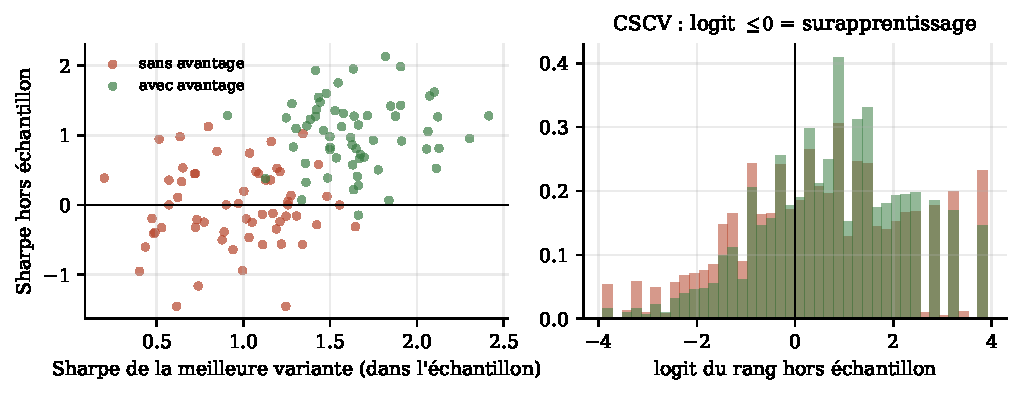
\includegraphics[width=0.95\textwidth]{ch16/is_oos_pbo.pdf}
\caption{À gauche, Sharpe de la meilleure variante dans l'échantillon contre hors échantillon (E4). À droite, distribution des logits de la CSCV (E5) : la masse à gauche de zéro est la PBO.}
\label{c16:fig:pbo}
\end{figure}

\paragraph{Lecture.} Dans le monde sans avantage, la PBO ($0{,}38$) est inférieure à $0{,}5$ alors que la meilleure variante ne gagne rien hors échantillon. La raison : la PBO mesure un \emph{classement relatif}. Les variantes à seuil élevé traitent moins et paient moins de coûts ; elles sont régulièrement \og moins mauvaises\fg{} que les autres, et cette régularité est réelle. La PBO dit donc si la sélection est reproductible, pas si la stratégie gagne. Elle se lit toujours avec le niveau du Sharpe hors échantillon et le DSR.

% =====================================================================
\section{Un moteur sans anticipation}
% =====================================================================

Le module \texttt{arbhub.backtest.engine} implémente les règles de ce chapitre en trois fonctions.

\begin{lstlisting}[language=Python]
from arbhub.backtest.engine import rolling_zscore, zscore_positions, pair_backtest
from arbhub.backtest.metrics import annualized_sharpe, deflated_sharpe, max_drawdown

z = rolling_zscore(y - beta * x, window=60)       # n'utilise que s[t-59..t]
q = zscore_positions(z, entry=2.0, exit=0.0, stop=4.0)
res = pair_backtest(y, x, beta, q, cost_bps=5)    # gain[t+1] = q[t] * dS ; couts en t
print(annualized_sharpe(res.net), max_drawdown(res.net), res.n_trades)
\end{lstlisting}

Les tests (\texttt{tests/test\_backtest.py}) vérifient : l'absence d'anticipation (modification des données futures) ; l'égalité du P\&L avec la formule manuelle~\eqref{c16:eq:pnl} ; des coûts payés uniquement lors des changements de position et égaux au notionnel échangé multiplié par le coût ; le fonctionnement du stop-loss ; l'égalité du \emph{z-score} glissant avec un calcul naïf ; et les propriétés de référence du PSR, du DSR et de la PBO.

% =====================================================================
\section{Les coûts, encore}
% =====================================================================

Un \emph{backtest} sans coûts est inutilisable (chapitres~1, 6 et~12). Le modèle minimal à déclarer, par jambe et par transaction : commission, demi-fourchette achat-vente, glissement estimé ; et, par jour de détention : coût d'emprunt des titres vendus à découvert, financement des positions à crédit, \emph{funding} des perpétuels (chapitre~14). Une bonne pratique est de publier le \emph{coût de rentabilité nulle} : le coût par jambe pour lequel le gain net devient nul. S'il est inférieur au double de vos coûts estimés, la stratégie n'a pas de marge de sécurité.

% =====================================================================
\section{Ce que la théorie apporte, et ses limites}
% =====================================================================

\paragraph{Apports.} Des ordres de grandeur sur ce qu'un \emph{backtest} peut prouver (il faut des années pour distinguer un Sharpe de 1 du hasard), une correction explicite du nombre d'essais, et un moteur dont l'absence d'anticipation est garantie par des tests.

\paragraph{Limites.} Le DSR et la PBO supposent que le passé est représentatif du futur ; aucun ne protège contre un changement de régime. Le nombre d'essais est souvent mal connu. Enfin, un \emph{backtest} ne capture pas l'exécution réelle (files d'attente, exécutions partielles, rejets) : seule une période de \emph{paper trading} puis de petite taille réelle mesure la stratégie telle qu'elle sera traitée (chapitre~18).

% =====================================================================
\section{Fiche à recopier au tableau blanc}
% =====================================================================

\begin{whiteboard}
\begin{itemize}[leftmargin=1.2em]
\item \textbf{Sans anticipation :} $\text{gain}_{t+1} = q_t(S_{t+1}-S_t)$, $q_t$ fonction des seules données $\le t$ ; test automatique : modifier le futur ne change pas le passé.
\item \textbf{Trois biais :} anticipation, survie (garder les radiés), sélection (compter les essais).
\item \textbf{Erreur-type du Sharpe :} $\sqrt{(1+SR^2/2)/T}$ par période ; annualisé $\approx 1/\sqrt{\text{années}}$.
\item \textbf{Maximum de $N$ Sharpe nuls :} $\approx\sqrt V\big((1-\gamma)\Phi^{-1}(1-\tfrac1N) + \gamma\Phi^{-1}(1-\tfrac{1}{Ne})\big)$, croît comme $\sqrt{2\ln N/T}$.
\item \textbf{PSR :} $\Phi\big((\widehat{SR}-SR^\ast)\sqrt{T-1}/\sqrt{1-\gamma_3\widehat{SR}+\frac{\gamma_4-1}{4}\widehat{SR}^2}\big)$ ; \textbf{DSR :} PSR avec $SR^\ast = \E[\max]$.
\item \textbf{PBO :} proportion des découpages CSCV où la meilleure variante en sélection finit sous la médiane en test.
\item \textbf{Découpage :} formation, validation, test regardé une seule fois ; \emph{walk-forward} ; purge et embargo.
\end{itemize}
\end{whiteboard}

% =====================================================================
\section{Exercices}
% =====================================================================

\begin{exercise}
Une stratégie affiche un Sharpe annualisé de $1{,}5$ sur deux ans de données quotidiennes. Calculez l'erreur-type et un intervalle de confiance à 95\,\% du vrai Sharpe. Combien d'années faudrait-il pour que la borne basse dépasse $0{,}5$ ?
\end{exercise}

\begin{exercise}
Vous avez testé 200 paires sur 4 ans et la meilleure affiche un Sharpe de $2{,}1$. En supposant $V = 1/T$, calculez le maximum espéré sous l'hypothèse nulle. Le résultat est-il impressionnant ?
\end{exercise}

\begin{exercise}
Démontrez l'approximation $\E[\max]\approx\sqrt{2V\ln N}$ pour $N$ grand, en utilisant $\Phi^{-1}(1-p)\approx\sqrt{2\ln(1/p)}$ pour $p$ petit.
\end{exercise}

\begin{exercise}[à coder]
Écrivez une fonction \texttt{walk\_forward(y, x, F, H)} qui réestime $\beta$, la moyenne et l'écart-type sur chaque fenêtre de formation de $F$ jours et trade les $H$ jours suivants. Ajoutez-lui un test d'absence d'anticipation dans \texttt{tests/}.
\end{exercise}

\begin{exercise}[à coder]
Remplacez dans E2 les rendements i.i.d. par des gains autocorrélés (AR(1) de paramètre $0{,}3$). De combien l'écart-type du Sharpe estimé augmente-t-il ? Comparez avec un \emph{bootstrap} par blocs de 20 jours.
\end{exercise}

\begin{exercise}[données réelles]
Reprenez votre meilleure paire du chapitre~7. Notez honnêtement combien de paires et de réglages vous avez essayés, puis calculez son DSR. Que concluez-vous ?
\end{exercise}

% =====================================================================
\section{Pour aller plus loin}
% =====================================================================

\begin{toread}
\begin{itemize}[leftmargin=1.2em]
\item \citet{bailey2014dsr} : sections 2 et 3 pour le maximum espéré et le DSR, avec un exemple numérique complet.
\item \citet{bailey2017pbo} : section 2 pour l'algorithme CSCV, section 4 pour l'interprétation de la PBO.
\item \citet{lo2002} : la loi asymptotique du Sharpe, y compris pour des rendements autocorrélés.
\item \citet{harvey2016} : sections sur les corrections de Bonferroni, Holm et Benjamini-Hochberg-Yekutieli.
\item \citet{white2000} : le \emph{reality check}, test formel de la meilleure parmi plusieurs stratégies.
\item \citet{lopezdeprado2018} : chapitres 7 (validation croisée purgée), 11 (dangers du \emph{backtest}) et 14 (statistiques de \emph{backtest}).
\end{itemize}
\end{toread}

\section{Scripts du chapitre}
\noindent\texttt{code/ch16/ch16\_backtest.py} : E1 (figure~\ref{c16:fig:lookahead}), E2, E3 (figure~\ref{c16:fig:emax}), E4–E5 (figure~\ref{c16:fig:pbo}), E6. Modules : \texttt{src/arbhub/backtest/engine.py}, \texttt{metrics.py} ; tests : \texttt{tests/test\_backtest.py}.
